\documentclass[10pt,a4paper,twocolumn]{article}

\usepackage[english]{babel}
\usepackage{float}
\usepackage{lipsum}

\input{pisika.dat}

%  Editorial staff will uncomment the next line
% \input{staff.hed}
\usepackage{tikz}
\usetikzlibrary{positioning, calc}

%% acronyms and glossary
\usepackage[
    single=true,
    sort=true,
    only-used=true
]{acro}
\DeclareAcronym{UWB}{
    short = UWB,
    long = Ultra-Wideband
}

\DeclareAcronym{TWR}{
    short = TWR,
    long = Two-Way Ranging
}

\DeclareAcronym{EKF}{
    short = EKF,
    long = Extended Kalman Filter
}

\DeclareAcronym{NLOS}{
    short = NLOS,
    long = Non-Line-Of-Sight
}

\DeclareAcronym{RTOS}{
    short = RTOS,
    long = Real-Time Operating System
}

\DeclareAcronym{TOF}{
    short = TOF,
    long = time-of-flight
}


%% Pictures
\renewcommand{\figurename}{Figure}

\begin{document}

%--------------------------------------------------------------------------
%  fill in the paper's title, author(s), and corresponding institutions
%--------------------------------------------------------------------------
\providecommand{\ShortAuthorList}[0]{S. Krebs, T. Herter} % use "A.~M.~Surname \textit{et al}." for more than three authors.
\title{Ultra-Wideband (UWB) Positioning System Based on ESP32 and DWM3000 Modules}
\author[1]{Sebastian Krebs}
\author[1]{Tom Herter}
\affil[1]{HTWG Konstanz,\linebreak  Faculty of Electronics und Informationtechnologies,\linebreak Germany}
%\affil[2]{Other Institute, XX University}

\date{\dateline{\today}}

\maketitle
\vspace*{-1.3cm}
%\thispagestyle{titlestyle}

\section*{}
%---------------------------------------------------------------------------
%               Include abstract and keywords here
%---------------------------------------------------------------------------
\textbf{\textit{Abstract}} - \textbf{
  In this paper, we introduce an innovative \ac{UWB} positioning system
  that leverages six identical custom-designed boards,
  each featuring an ESP32 microcontroller and integrated with DWM3000
  modules from Quorvo.}

  \textbf{This system is capable of achieving precise localization through \ac{TWR}
  measurements between one designated ''Tag'' board and five other ''Anchor'' boards.
  The collected distance measurements are processed by an \ac{EKF} running locally
  on the Tag board, enabling it to determine its own position with high accuracy,
  relying on the fixed positions of the Anchor boards.}

  \textbf{This paper presents a comprehensive overview of the system's architecture,
  the key components, and the remarkable capabilities it offers for accurate
  indoor positioning and tracking applications.}

\vspace*{.28cm}
\keywords{\textbf{RTLS, UWB, TOF, Positioning, Tracking}}

%---------------------------------------------------------------------------
%               the main text of your paper begins here
%---------------------------------------------------------------------------

\section{Introduction}\label{section:intro}
Indoor positioning and tracking have gained significant importance in various domains,
including logistics, healthcare, industrial automation, and smart infrastructure.
Traditional positioning systems often face challenges in terms of accuracy, scalability,
and robustness.
To address these issues, we present an \ac{UWB} positioning system that capitalizes
on advanced hardware and sophisticated algorithms,
resulting in an exceptional level of accuracy and reliability.

Our \ac{UWB} system comprises six identical boards,
all based on the ESP32 microcontroller, a versatile and powerful platform known
for its capabilities in wireless communication and processing.
These boards are equipped with DWM3000 modules from Quorvo,
renowned for their high-performance UWB capabilities.

One of these boards is designated as the ''Tag'',
responsible for initiating \ac{TWR} measurements with the remaining five ''Anchor'' boards.
The innovative aspect of our system lies in its ability to perform accurate localization
without reliance on external infrastructure or centralized processing.

The heart of our UWB system is the \ac{EKF} implemented locally on the Tag board.
This EKF takes the distance measurements obtained from TWR with the Anchor boards and,
based on their known fixed positions, computes the real-time position of the Tag board
with remarkable precision.
This decentralized approach not only ensures rapid and reliable positioning but also
offers scalability, making it suitable for various applications where real-time location
data is crucial.

In this paper, we will delve into the details of our \ac{UWB} system,
explaining the hardware setup as well as the firmware architecture.

\section{Measurement Priciple}\label{Section:principle}
\acf{TWR} is our foundational technique for obtaining precise distance
measurements within the UWB positioning system.
It relies on the time it takes for signals to travel from a Tag board to Anchor boards
and back again.
This temporal measurement, in compliance with the IEEE 802.15.4a/4z standards,
offers the basis for distance estimation.

The following Figure \ref{fig:twr} shows how a
\ac{TWR} Handschake is done.
The Tag Firmware calculates the time-of-flight aswell
as the distance between both devices by comparing the
timestamps of sending and reception.

\begin{figure}[H]
  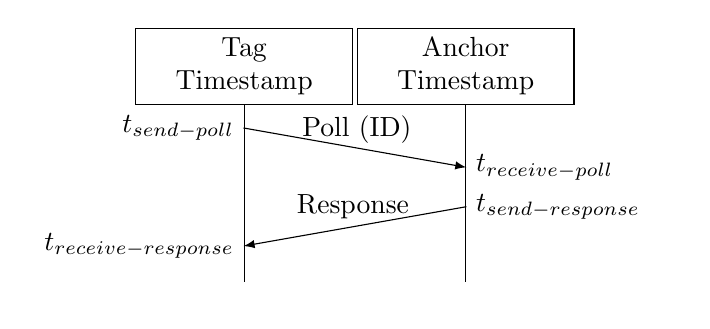
\begin{tikzpicture}[
    node distance=1.5cm,
    block/.style={
      align=center, draw,minimum width=2.75cm, minimum height=.5cm
    },
    ghost/.style={
      align=center,minimum width=0cm, minimum height=0cm
    },
    label/.style={
      minimum width=2cm, minimum height=0cm, text width=2.5cm
    },
    >=latex,
  ]
    % textfields
    \node [block] (tag_timestamp) {Tag\\Timestamp};
    \node [block, right=.05cm of tag_timestamp] (anchor_timestamp) {Anchor\\Timestamp};

    % Endpoints
    \node [ghost, below=2.25cm of tag_timestamp] (tag_endpoint) {};
    \node [ghost, below=2.25cm of anchor_timestamp] (anchor_endpoint) {};

    % Timelines
    \draw [-] (tag_timestamp) -- (tag_endpoint);
    \draw [-] (anchor_timestamp) -- (anchor_endpoint);

    % Labels Tag-line
    \node [label, align=right, anchor=east, below=.5cm of tag_timestamp.west] (t_send_poll) {$t_{send-poll}$};
    \node [label, align=right, anchor=east, below=2cm of tag_timestamp.west] (t_receive_response) {$t_{receive-response}$};
    
    % Labels Anchor-line
    \node [label, align=left, anchor=west, below=1cm of anchor_timestamp.east] (t_receive_poll) {$t_{receive-poll}$};
    \node [label, align=left, anchor=west, below=1.5cm of anchor_timestamp.east] (t_send_response) {$t_{send-response}$};

    %Dotted lines
    \draw [->] (t_send_poll.east) -- (t_receive_poll.west);
    \draw [->] (t_send_response.west) -- (t_receive_response.east);
    \node [ghost, below=.5cm of anchor_timestamp.west] (poll_label) {Poll (ID)};
    \node [ghost, below=1.5cm of tag_timestamp.east] (response_label) {Response};

  \end{tikzpicture}
  \caption{Timingdiagram of \acf{TWR}}
  \label{fig:twr}
\end{figure}

For in-depth technical specifications and methodologies,
we direct interested readers to explore the IEEE 802.15.4a/4z
standards documentation \cite{IEEE802154a} \cite{IEEE802154z},
which provides comprehensive guidelines for the
intricate orchestration of UWB signals and the calculation of time-of-flight.
These standards ensure the rigor and accuracy of our distance measurements,
forming the cornerstone of our UWB-based positioning and tracking capabilities.

\section{System Architecture}\label{section:system_arch}
In our scenario, five Anchors are strategically distributed throughout the room,
positioned at a height on the ceiling to minimize the likelihood of 
\ac{NLOS} conditions.
These five Anchors do not possess information specific to their usage.

Customized settings, such as Anchor positions,
can be transmitted to the Tag within our designed system through a BLE interface.
The Tag leverages these provided Anchor positions,
in conjunction with distance measurements,
to determine its own position accurately.

The following diagram elucidates the interactions among the individual components.
It becomes evident that when selecting Anchor positions,
particular emphasis should be placed on ensuring uniform distribution along all three axes.
Additionally, an overhead perspective aids in mitigating measurement inaccuracies.

\begin{figure}[H]
  \centering
  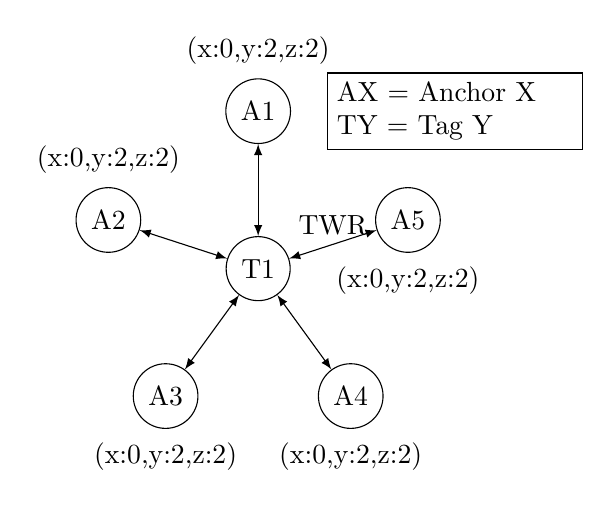
\begin{tikzpicture}[
    node distance=1.5cm,
    device/.style={
      align=center, circle, draw, minimum width=.25cm, minimum height=.5cm
    },
    ghost/.style={
      align=center,minimum width=0cm, minimum height=0cm
    },
    label/.style={
      draw, minimum width=2cm, minimum height=0cm, text width=3cm
    },
    >=latex,
  ]
    % Responders with coords
    \node [device] (device2) at (90:2cm) {A1};
    \node [ghost, above=.05cm of device2.north] (dev2) {(x:0,y:2,z:2)};
    \node [device] (device3) at (162:2cm) {A2};
    \node [ghost, above=.05cm of device3.north] (dev3) {(x:0,y:2,z:2)};
    \node [device] (device4) at (234:2cm) {A3};
    \node [ghost, below=.05cm of device4.south] (dev4) {(x:0,y:2,z:2)};
    \node [device] (device5) at (306:2cm) {A4};
    \node [ghost, below=.05cm of device5.south] (dev5) {(x:0,y:2,z:2)};
    \node [device] (device6) at (18:2cm) {A5};
    \node [ghost, below=.05cm of device6.south] (dev6) {(x:0,y:2,z:2)};

    %Initiator
    \node [device] (device1) at (0,0) {T1};

    % TWRs
    \draw [<->] (device1) -- (device2); 
    \draw [<->] (device1) -- (device3); 
    \draw [<->] (device1) -- (device4); 
    \draw [<->] (device1) -- (device5); 
    \draw [<->] (device1) -- node[midway, above, align=left] {TWR} (device6);

    %legend
    \node [label] (legend) at (2.5,2) {AX = Anchor X \\TY = Tag Y};

  \end{tikzpicture}
  \caption{Systemarchitecture for Positioning}
  \label{fig:systemarch}
\end{figure}

This strategic approach to Anchor placement not only optimizes
our positioning system's performance but also reduces the potential
for measurement errors.

\section{Hardware Design}\label{section:hardware}
The hardware design of our system draws inspiration from pre-existing DWM3000 Evaluation
boards.
However, our proprietary board development enables specialized component selection
tailored to their intended use cases.
User-friendliness was a paramount consideration during the design process,
resulting in the integration of multiple user buttons and LEDs.
Additionally, the PCB incorporates a convenient LiPo battery charging capability
via USB-C.

Notably, our PCB design ensures a consistent layout across all boards,
regardless of their specific application.
Below the antennas of both the DWM3000 and ESP32,
the ground plate has been selectively omitted to enhance antenna radiation
characteristics and enable more precise measurements.
This meticulous hardware design approach not only optimizes
performance but also prioritizes user convenience. 

\section{Firmware Architecture}\label{section:firmware}
To meet the demanding timing requirements essential for \ac{TOF}
measurements and enhance network round-trip times,
our firmware is implemented based on a \ac{RTOS}.
FreeRTOS \cite{FreeRTOS_2023}, in particular,
offers the capability to create multiple tasks that collaborate coherently
and can be executed simultaneously on each of the two cores of the ESP32 microcontroller.

In the regular tracking mode,
all devices within the system execute the TOF task, ensuring synchronized data acquisition.
When a device is configured as a Tag,
it additionally undertakes the execution of the \ac{EKF} task.
The EKF task processes the distance measurements generated by the TOF task,
culminating in a precise positional estimation.

\subsection{TOF-Task}\label{section:firmware-tof}
The \ac{TOF} task within our system takes its cues from the example code
provided by Quorvo for Two-Way Ranging (TWR) measurements.
However, we've refined the functionality by structuring it within a class-based framework.
The commonalities shared between the initiator and responder roles have
been encapsulated within a shared superclass.
This design choice allows us to maintain a streamlined and concise software structure,
reducing redundancy and simplifying maintenance.

In practice, the Tag, which acts as the TWR initiator,
iterates through a list of Anchors, each serving as a TWR responder.
The Tag orchestrates distance measurements with each Anchor,
resulting in a comprehensive dataset that serves as the basis for
precise indoor localization.

\subsection{EKF-Task}\label{section:firmware-ekf}
The \ac{EKF} employed in our system leverages two distinct mathematical models
to achieve precise position estimation.
For readers interested in delving deeper into the theoretical foundations of the
Kalman Filter, we recommend consulting the work of Li Qiang et al. in
"Kalman Filter and Its Application"~\cite{Kalman}.
The EKF  on the Tag utilizes a prediction model based on the constant velocity model assumption.
It posits that the tracked object moves with a consistent velocity along its recent
trajectory.
This model serves as a fundamental tool for forecasting the future position of the tag.

The measurement model is encapsulated in Equation~\ref{eq:measurementmatrix},
enabling the transformation of measured distances into accurate position estimations.
The measurement model finds its expression in the measurement matrix $H$,
which effectively links the measured distances to the position estimation:
\begin{equation}
  \begin{aligned}
    \Delta x_i &= x_i - x \\
    \Delta y_i &= y_i - y \\
    \Delta z_i &= z_i - z \\
    dist_i &= \sqrt{{\Delta x_i^2 + \Delta y_i^2 + \Delta z_i^2}} \\
    H &= \begin{bmatrix}
    -\frac{{\Delta x_1}}{{dist_1}} & -\frac{{\Delta y_1}}{{dist_1}} & -\frac{{\Delta z_1}}{{dist_1}} \\
    -\frac{{\Delta x_2}}{{dist_2}} & -\frac{{\Delta y_2}}{{dist_2}} & -\frac{{\Delta z_2}}{{dist_2}} \\
    \vdots & \vdots & \vdots \\
    -\frac{{\Delta x_{\text{max}}}}{{dist_{\text{max}}}} & -\frac{{\Delta y_{\text{max}}}}{{dist_{\text{max}}}} & -\frac{{\Delta z_{\text{max}}}}{{dist_{\text{max}}}}
    \end{bmatrix}
  \end{aligned}
  \label{eq:measurementmatrix}
\end{equation}
This matrix, $H$, plays a crucial role in incorporating distance measurements
into the state estimation process, a core facet of the EKF algorithm.

\section{Test Results}\label{section:tests}
\textbf{Need to do some}

\section{Conclusion And Outlook}\label{section:conclusion}
\textbf{Need to conclude something}

Additionally, we are committed to fostering collaboration and knowledge-sharing
within the community.
Therefore, we have made the entire source code, along with all PCB design files,
readily accessible to the public.
You can find these resources, along with detailed documentation,
on our project's GitHub repository \cite{uwb-tracking}.


% Please use pisikabst.bst. You may your own *.bib file.
\bibliographystyle{pisikabst}
\bibliography{bibliography}

\end{document}